\section*{Supplementary Note 6. The social cognitive theory model: the motivating case}

The method was conceived while estimating a dynamical model of Bandura's social cognitive theory (SCT) of physical activity from the daily records of one participant (Miranda et al., 2025 IEEE Ecuador Technical Chapters Meeting, doi:10.1109/ETCM67548.2025.11304524; cited in the main text). This note documents that case. It is not part of the PEtab benchmark (it is not an SBML/PEtab problem and its data are not public), it is not counted in any benchmark statistic, and its model was not translated into Lean; it is reported because it shows, on a small model with real data, the problem that the method addresses.

\subsection*{Model and data}
Six psychosocial constructs $x_1,\dots,x_6$, of which $x_4$ is behaviour (daily steps), evolve as a linear system $\tau_i\dot x_i=-x_i+\sum_j\beta_{ij}x_j+\sum_k\gamma_{ik}u_k$, i.e.\ $\dot x=A(\theta)x+B(\theta)u$, $y=x_4$, with ten couplings $\beta_{14},\beta_{21},\beta_{25},\beta_{31},\beta_{34},\beta_{42},\beta_{43},\beta_{45},\beta_{46},\beta_{54}$, six input gains $\gamma_{33},\gamma_{35},\gamma_{36},\gamma_{57},\gamma_{64},\gamma_{68}$ ($\gamma_{35}$ with negative sign) and six time constants $\tau_1,\dots,\tau_6$: 22 parameters. The data are 31 days of six measured inputs and daily steps, each standardised (z-score). The model is simulated from $x(0)=0$ with inputs held constant over each day (exact discretisation with the matrix exponential), and the output of day $k$ is $x_4$ at the end of that day. Bounds are $\beta\in[-1.5,1.5]$, $\gamma\in[0,3]$, $\tau\in[0.3,12]$, and only parameter values with stable dynamics ($\max\operatorname{Re}\lambda(A)\le-10^{-3}$) are admitted.

\subsection*{The problem that motivated the method}
In that study, differential evolution reached $R^2=86.11\%$, but local refinement from that estimate with a Levenberg--Marquardt grey-box method reached only 11\% and, after 20 recursive iterations, 41.17\%: different parameter sets fitted the data with very different quality, and gradient-based refinement was unreliable. The estimate used here as $\theta_0$ was obtained with the same differential-evolution framework, with stability enforced and couplings of either sign (seed 2026, $R^2=0.881$). Repeating the search with 100 seeds gave fits of essentially the same quality ($R^2$ between 0.878 and 0.884) with very different parameters: 8 of the ten couplings change sign between runs, and most parameters span almost their whole admissible range (Table~S7). The data cannot separate the parameters, and fitting all 22 of them is ill-posed. Deciding which few parameters the data can inform, before fitting, is the question that the method answers.

{\small
\begin{longtable}{@{}lrrrrc@{}}
\caption*{\textbf{Supplementary Table S7.} Parameters of the SCT model: value at $\theta_0$, range over the 100 differential-evolution runs (all with $R^2\ge0.87$), sign change between runs, and share of the sensitivity energy $E_j/\sum_kE_k$ of behaviour at $\theta_0$.}\\
\toprule
Parameter & $\theta_0$ & min & max & Energy share & Sign change \\
\midrule
\endhead
$\beta_{14}$ & 0.628 & -1.49 & 1.47 & 0.4\% & yes \\
$\beta_{21}$ & 1.09 & -1.49 & 1.43 & 0.4\% & yes \\
$\beta_{25}$ & 0.333 & -1.46 & 1.47 & 0.1\% & yes \\
$\beta_{31}$ & 0.74 & -1.48 & 1.29 & 0.0\% & yes \\
$\beta_{34}$ & -0.756 & -1.47 & 1.27 & 0.0\% & yes \\
$\beta_{42}$ & 1.08 & -1.43 & 1.49 & 0.5\% & yes \\
$\beta_{43}$ & 0.00603 & -0.508 & 0.543 & 0.0\% & yes \\
$\beta_{45}$ & 1.36 & 0.809 & 1.5 & 27.0\% & -- \\
$\beta_{46}$ & 0.247 & -1.49 & 1.46 & 0.0\% & yes \\
$\beta_{54}$ & -0.732 & -1.5 & -0.561 & 8.5\% & -- \\
$\gamma_{33}$ & 2.91 & 0.00653 & 2.91 & 0.0\% & -- \\
$\gamma_{35}$ & 1.03 & 9.3e-04 & 2.98 & 0.0\% & -- \\
$\gamma_{36}$ & 1.49 & 0.0126 & 2.97 & 0.0\% & -- \\
$\gamma_{57}$ & 1.42 & 1.08 & 2.84 & 46.2\% & -- \\
$\gamma_{64}$ & 0.519 & 0.0832 & 3 & 0.0\% & -- \\
$\gamma_{68}$ & 0.571 & 0.00602 & 2.89 & 0.0\% & -- \\
$\tau_{1}$ & 5.71 & 0.36 & 11.5 & 0.1\% & -- \\
$\tau_{2}$ & 4.82 & 0.469 & 11.1 & 0.1\% & -- \\
$\tau_{3}$ & 8.67 & 0.606 & 12 & 0.0\% & -- \\
$\tau_{4}$ & 0.462 & 0.308 & 1.05 & 7.0\% & -- \\
$\tau_{5}$ & 0.578 & 0.327 & 1.03 & 9.7\% & -- \\
$\tau_{6}$ & 10.9 & 0.609 & 12 & 0.0\% & -- \\
\bottomrule
\end{longtable}
}

\subsection*{What the method finds}
\textbf{Collinearity.} The sensitivity matrix of behaviour at $\theta_0$ is exactly rank-deficient (infinite condition number, largest VIF $4.5\times10^{15}$), and 9 pairs of parameters have sensitivity vectors with cosine $\ge0.95$, for example $\beta_{14}$--$\beta_{21}$ (1.000), $\tau_{4}$--$\tau_{5}$ (0.997), $\beta_{34}$--$\beta_{42}$ (0.984), $\beta_{14}$--$\beta_{31}$ (0.965).

\textbf{Selection.} Stage~1 reached $R_{\mathrm{var}}=74\%$ with 7 parameters, below the threshold of 89\% because the remaining candidates failed the conditioning test; stage~2 selected two parameters, $\gamma_{57}$ and $\beta_{45}$ (condition number 4.2, VIF 5.0), which form the path from the external input through construct $x_5$ to behaviour and together carry 73\% of the sensitivity energy. The conditioning test rejected redundant candidates such as $\tau_4$ and $\tau_5$, strongly collinear with $\beta_{45}$ (cosine about 0.8). Backward elimination removed nothing.

\textbf{Admissibility and robustness.} Re-estimating only these two parameters reproduces the output of the full model with a median $e_{\mathrm{fit}}$ of 11.4\% at $\pm5\%$, and between 10.6\% and 15.1\% for perturbations up to $\pm50\%$ (pattern A). The median $\cos\Delta$ is 0.94 and $R_{\mathrm{var}}=0.73$, so the subset reaches level 2 of the guarantees defined in Supplementary Table~S1.

\textbf{Prediction of unseen days.} Both models were refitted to days 1--24 (by least squares from $\theta_0$, within the bounds and with the stability constraint) and used to predict days 25--31 (Figure~S2). The reduced model predicted the held-out week with $R^2=0.84$ (test $\chi^2/n$ 1.63), better than the full 22-parameter model ($R^2=0.67$, $\chi^2/n$ 3.44; refitted with the same differential-evolution search: $R^2=0.79$, $\chi^2/n$ 2.13), even though the full model fits the training days more closely ($\chi^2/n$ 0.65 versus 0.84). All refitted models are stable.

\begin{figure}[!htb]
\centering
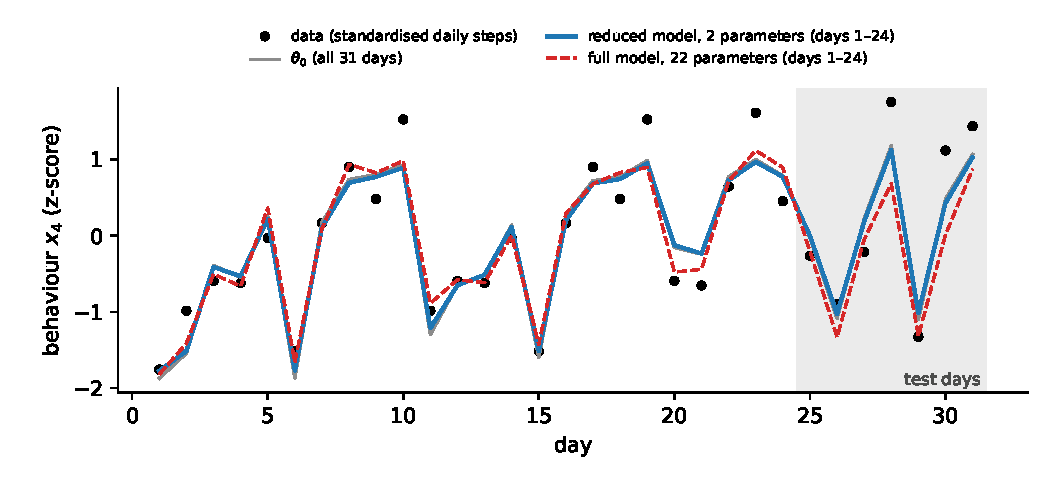
\includegraphics[width=\textwidth]{figures/figS2_sct.pdf}
\caption*{\textbf{Supplementary Figure S2. SCT model of one participant.} Standardised daily steps (dots), the fit of $\theta_0$ to all 31 days (grey), and the reduced (two parameters, blue) and full (22 parameters, red dashed) models refitted to days 1--24; the shaded region contains the seven test days.}
\end{figure}

\subsection*{Relation with the formal results}
The SCT model is linear with constant inputs on each day, so its vector field is globally Lipschitz and the existence and differentiability results of Part~II of Supplementary Note~2 apply directly; the model was not translated into Lean, so this is a mathematical observation rather than a machine-checked statement. The model shows on a small, transparent example the situation that the method is designed for: a good fit of the data, parameters that the data cannot determine, and a reduced set of two parameters that reproduces and predicts the measured behaviour.

